% ============================================================
%  يُترجَم بـ XeLaTeX  (في Overleaf: Menu → Compiler → XeLaTeX)
%  الخط: Amiri (متوفر في Overleaf، أو حمّله من github.com/aliftype/amiri)
% ============================================================
\documentclass[12pt,a4paper]{article}
\usepackage[a4paper,margin=1.2cm,top=2.3cm,bottom=2.9cm,headheight=15pt,footskip=1.5cm]{geometry}
\usepackage{amsmath,amssymb}
\usepackage{icomma}
\usepackage[english,bidi=default,layout=lists]{babel}
\babelprovide[import,main]{arabic}
\babelfont{rm}[Scale=1.08]{Amiri}
\babelfont{sf}[Scale=1.08]{Amiri}
\usepackage[most]{tcolorbox}
\usepackage{tikz}
\usetikzlibrary{arrows.meta,calc,shadings}
\usepackage{array}
\usepackage{colortbl}
\usepackage{fancyhdr}
\usepackage{titlesec}
\usepackage{enumitem}
\usepackage{collcell}
\usepackage{needspace}
\usepackage{etoolbox}
\newcolumntype{C}{>{\collectcell\ar}c<{\endcollectcell}}
\pretocmd{\section}{\Needspace{15\baselineskip}}{}{}
\pretocmd{\subsection}{\Needspace{11\baselineskip}}{}{}

\definecolor{cDef}{HTML}{1F4E9C}
\definecolor{cThm}{HTML}{B3261E}
\definecolor{cRem}{HTML}{2E7D32}
\definecolor{cEx}{HTML}{C76B00}
\definecolor{cMeth}{HTML}{6A1B9A}
\definecolor{cSol}{HTML}{00695C}
\definecolor{cSec}{HTML}{1F3A68}

\titleformat{\section}{\Large\bfseries\color{cSec}}{\thesection.}{0.6em}{}[{\color{cSec!60}\titlerule[1pt]}]
\titleformat{\subsection}{\large\bfseries\color{cThm!85!black}}{\thesubsection.}{0.5em}{}
\titlespacing*{\section}{0pt}{14pt}{8pt}
\titlespacing*{\subsection}{0pt}{10pt}{5pt}
\setlength{\parindent}{0pt}
\setlength{\parskip}{4pt}
\setlist{itemsep=2pt,topsep=3pt}

\newtcolorbox{arbox}[3][]{enhanced,
  colback=#2!5,colframe=#2!80!black,arc=2mm,boxrule=0.8pt,
  left=6pt,right=6pt,top=8pt,bottom=5pt,
  fonttitle=\bfseries,coltitle=white,
  title={\foreignlanguage{arabic}{#3}},
  attach boxed title to top right={xshift=-5mm,yshift=-3mm},
  boxed title style={colback=#2!80!black,arc=1.5mm,boxrule=0pt},
  before upper={\selectlanguage{arabic}},
  before skip=8pt,after skip=8pt,breakable,#1}
\newenvironment{BOX}[2]{\begin{otherlanguage}{english}\begin{arbox}{#1}{#2}}{\end{arbox}\end{otherlanguage}}
\newenvironment{tarif}[1][تعريف]{\begin{BOX}{cDef}{#1}}{\end{BOX}}
\newenvironment{khassia}[1][خاصية]{\begin{BOX}{cThm}{#1}}{\end{BOX}}
\newenvironment{molahada}[1][ملاحظة]{\begin{BOX}{cRem}{#1}}{\end{BOX}}
\newenvironment{mithal}[1][مثال]{\begin{BOX}{cEx}{#1}}{\end{BOX}}
\newenvironment{tariqa}[1][طريقة]{\begin{BOX}{cMeth}{#1}}{\end{BOX}}

\newcounter{exo}
\newenvironment{tamrin}[1]{\stepcounter{exo}\begin{BOX}{cSec}{التمرين \theexo: #1}}{\end{BOX}}
\newenvironment{hal}{\Needspace{12\baselineskip}\begin{otherlanguage}{english}\begin{arbox}[breakable]{cSol}{حل التمرين \theexo}}{\end{arbox}\end{otherlanguage}}

\newenvironment{LTR}{\begin{otherlanguage}{english}}{\end{otherlanguage}}
\newcommand{\ar}[1]{\foreignlanguage{arabic}{#1}}

\renewcommand{\dots}{\mathinner{\ldotp\ldotp\ldotp}}
\renewcommand{\ldots}{\mathinner{\ldotp\ldotp\ldotp}}
\renewcommand{\cdots}{\mathinner{\cdotp\cdotp\cdotp}}
\newcommand{\N}{\mathbb{N}}
\newcommand{\Z}{\mathbb{Z}}
\newcommand{\D}{\mathbb{D}}
\newcommand{\Q}{\mathbb{Q}}
\newcommand{\R}{\mathbb{R}}
\newcommand{\pgcd}{\operatorname{PGCD}}
\newcommand{\ppcm}{\operatorname{PPCM}}

% \NLseg{a}{b}{[}{]} ; \NLright{a}{[} ; \NLleft{b}{]}  (interval on a number line)
\newcommand{\NLseg}[4]{\begin{LTR}\begin{tikzpicture}[baseline=-0.6ex]
 \draw[-{Stealth[length=2mm]},gray!70](0,0)--(3.4,0);
 \draw[line width=2pt,cThm!80!black](0.7,0)--(2.7,0);
 \node[cThm!80!black,font=\LARGE] at (0.7,0){$#3$};
 \node[cThm!80!black,font=\LARGE] at (2.7,0){$#4$};
 \node[below=3pt,font=\footnotesize] at (0.7,0){$#1$};
 \node[below=3pt,font=\footnotesize] at (2.7,0){$#2$};
\end{tikzpicture}\end{LTR}}
\newcommand{\NLright}[2]{\begin{LTR}\begin{tikzpicture}[baseline=-0.6ex]
 \draw[-{Stealth[length=2mm]},gray!70](0,0)--(3.4,0);
 \draw[line width=2pt,cThm!80!black](1.3,0)--(3.3,0);
 \node[cThm!80!black,font=\LARGE] at (1.3,0){$#2$};
 \node[below=3pt,font=\footnotesize] at (1.3,0){$#1$};
\end{tikzpicture}\end{LTR}}
\newcommand{\NLleft}[2]{\begin{LTR}\begin{tikzpicture}[baseline=-0.6ex]
 \draw[-{Stealth[length=2mm]},gray!70](0,0)--(3.4,0);
 \draw[line width=2pt,cThm!80!black](0.05,0)--(2.1,0);
 \node[cThm!80!black,font=\LARGE] at (2.1,0){$#2$};
 \node[below=3pt,font=\footnotesize] at (2.1,0){$#1$};
\end{tikzpicture}\end{LTR}}

% ---------- social-media icons (pure TikZ) ----------
\definecolor{cFB}{HTML}{1877F2}
\definecolor{cTG}{HTML}{229ED9}
\definecolor{cIG1}{HTML}{FEDA75}
\definecolor{cIG2}{HTML}{D62976}
\definecolor{cIG3}{HTML}{4F5BD5}
\newcommand{\fbicon}{\begin{LTR}\begin{tikzpicture}[baseline=-0.75ex,x=1em,y=1em]
 \fill[cFB] (0,0) circle (0.55);
 \node[white,inner sep=0,font=\usefont{TU}{lmss}{bx}{n}\small] at (0.04,-0.02) {f};
\end{tikzpicture}\end{LTR}}
\newcommand{\igicon}{\begin{LTR}
\begin{tikzpicture}[baseline=-0.75ex,x=1em,y=1em]
 \shade[lower left=cIG1,lower right=cIG2,upper left=cIG2,upper right=cIG3,rounded corners=0.28em] (-0.55,-0.55) rectangle (0.55,0.55);
 \draw[white,line width=0.09em,rounded corners=0.18em] (-0.36,-0.36) rectangle (0.36,0.36);
 \draw[white,line width=0.09em] (0,0) circle (0.17);
 \fill[white] (0.22,0.22) circle (0.05);
\end{tikzpicture}\end{LTR}}
\newcommand{\tgicon}{\begin{LTR}
\begin{tikzpicture}[baseline=-0.75ex,x=1em,y=1em]
 \fill[cTG] (0,0) circle (0.55);
 \fill[white] (-0.33,0.0) -- (0.32,0.27) -- (0.2,-0.3) -- (0.0,-0.15) -- (-0.08,-0.28) -- (-0.08,-0.08) -- cycle;
 \fill[cTG!70!black] (-0.08,-0.08) -- (0.25,0.2) -- (0.0,-0.15) -- (-0.08,-0.28) -- cycle;
\end{tikzpicture}\end{LTR}}
% page number: black box, white two-digit number, at the right of the social row
\newcommand{\PageBox}{\begin{LTR}\tikz[baseline=(p.base)]\node[fill=black,text=white,inner sep=2.5pt,minimum width=1.6em,minimum height=1.3em,font=\usefont{TU}{lmss}{bx}{n}\small](p){\ifnum\value{page}<10 0\fi\arabic{page}};\end{LTR}}
% visual left-to-right order: Telegram | Instagram | Facebook | page box
\newcommand{\SocialRow}{\begin{otherlanguage}{english}%
 \ar{\textbf{الأستاذ سوايسية هشام للرياضيات}}\ \tgicon\hfill
 \textbf{prof\_hicham\_math}\ \igicon\hfill
 \ar{\textbf{الأستاذ سوايسية هشام للرياضيات}}\ \fbicon\hspace{2.2em}\PageBox\end{otherlanguage}}

\pagestyle{fancy}
\fancyhf{}
\renewcommand{\headrulewidth}{0.6pt}
\renewcommand{\footrulewidth}{0.4pt}
% \SetHeader{right head: document title}{left head: level -- stream}
\newcommand{\SetHeader}[2]{%
 \fancyhead[C]{\parbox{\textwidth}{\ar{#1\hfill #2}}}%
 \fancyfoot[C]{\parbox{\textwidth}{\small\SocialRow}}}
\usepackage{tkz-tab}
\usepackage{multicol}
% variation / sign table (LTR)
\newenvironment{TAB}{\par\begin{center}\begin{LTR}\begin{tikzpicture}[scale=0.95,every node/.style={font=\small}]}{\end{tikzpicture}\end{LTR}\end{center}}
% grid + axes, clipped: \begin{GR}{xmin}{xmax}{ymin}{ymax}{unit cm}
\newenvironment{GR}[5]{\par\begin{center}\begin{LTR}\begin{tikzpicture}[x=#5cm,y=#5cm,font=\footnotesize]
 \draw[gray!25,very thin] (#1,#3) grid (#2,#4);
 \draw[-{Stealth[length=2mm]}] (#1,0)--(#2+0.3,0) node[below left]{$x$};
 \draw[-{Stealth[length=2mm]}] (0,#3)--(0,#4+0.3) node[below left]{$y$};
 \node[below left] at (0,0){$O$};
 \begin{scope}\clip (#1,#3) rectangle (#2,#4);}
{\end{scope}\end{tikzpicture}\end{LTR}\end{center}}
\newcommand{\Ticks}[2]{\foreach \t in {#1} \node[below,font=\scriptsize] at (\t,0){$\t$}; \foreach \t in {#2} \node[left,font=\scriptsize] at (0,\t){$\t$};}
\newcommand{\bx}[1]{\ensuremath{\colorbox{cDef!12}{$\displaystyle #1$}}}
\newcommand{\TwoCol}[4]{\par\begin{LTR}\noindent\begin{minipage}[t]{#1\textwidth}\selectlanguage{arabic}#2\end{minipage}\hfill\begin{minipage}[t]{#3\textwidth}\selectlanguage{arabic}#4\end{minipage}\end{LTR}\par}
\newcommand{\RL}[4]{\TwoCol{#3}{#4}{#1}{#2}}  % \RL{w1}{right content}{w2}{left content}
\newcommand{\ok}{$\textcolor{cRem}{\checkmark}$}
\newcommand{\limn}{\displaystyle\lim_{n\to+\infty}}
% sub-questions, each on its own line
\newenvironment{sq}{\begin{itemize}[leftmargin=2.4em,itemsep=3pt]}{\end{itemize}}
\newcommand{\qa}{\item[(أ)]}\newcommand{\qb}{\item[(ب)]}\newcommand{\qc}{\item[(جـ)]}\newcommand{\qd}{\item[(د)]}\newcommand{\qe}{\item[(هـ)]}
\newcommand{\pa}{\par\smallskip\textbf{(أ)} }\newcommand{\pb}{\par\smallskip\textbf{(ب)} }\newcommand{\pc}{\par\smallskip\textbf{(جـ)} }\newcommand{\pd}{\par\smallskip\textbf{(د)} }\newcommand{\pe}{\par\smallskip\textbf{(هـ)} }
\newcommand{\QQ}[1]{\par\smallskip\textbf{#1.} }
\newenvironment{tmr}{\stepcounter{exo}\begin{BOX}{cSec}{تمرين محلول \theexo}}{\end{BOX}}
\newcommand{\ABC}[3]{\\[2pt]\begin{tabular}{p{0.28\textwidth}p{0.28\textwidth}p{0.28\textwidth}}(جـ) \ #3 & (ب) \ #2 & (أ) \ #1\end{tabular}}
\pretocmd{\section}{\Needspace{24\baselineskip}}{}{}
\newtcbox{\bxtbox}{on line,colback=cDef!12,colframe=cDef!12,boxrule=0pt,arc=1pt,boxsep=0pt,left=2pt,right=2pt,top=1pt,bottom=1pt}
\newcommand{\bxt}[1]{\foreignlanguage{english}{\bxtbox{\ar{#1}}}}
\usepackage{longtable}
\setlength{\LTpre}{4pt}\setlength{\LTpost}{0pt}
\newcommand{\Phase}[1]{\textbf{#1}}
\newcommand{\Fld}[2]{\textbf{#1:}\ #2}
% رأس المذكرة على نمط النموذج: إطار بعنوان «مذكرة رقم»، معلومات الحصة، ثم إطار الكفاءات
\newcommand{\ModhHead}[9]{%
\begin{LTR}
\begin{tcolorbox}[enhanced,colback=white,colframe=cThm!85!black,arc=4mm,boxrule=1pt,top=14pt,bottom=6pt,left=8pt,right=8pt,
 overlay={\node[fill=cThm!85!black,text=white,rounded corners=3mm,inner xsep=14pt,inner ysep=4pt,font=\large\bfseries] at ([yshift=0pt]frame.north){\ar{مذكرة رقم #1}};},
 before upper={\selectlanguage{arabic}}]
\begin{tabular}{@{}p{0.4\linewidth}p{0.55\linewidth}@{}}
\Fld{المستوى}{#2} & \Fld{الثانوية}{\dotfill}\\[3pt]
\Fld{المادة}{رياضيات} & \Fld{ميدان التعلم}{#3}\\[3pt]
\Fld{المدة}{#5} & \Fld{الوحدة التعلمية}{#4}\\[3pt]
\Fld{الأستاذ}{\dotfill} & \Fld{المحتوى المعرفي}{#6}\\
\end{tabular}
\end{tcolorbox}
\begin{tcolorbox}[enhanced,colback=white,colframe=cThm!85!black,arc=3mm,boxrule=0.8pt,sidebyside,sidebyside align=top,lefthand ratio=0.5,
 segmentation style={dashed,cThm!60},before upper={\selectlanguage{arabic}},before lower={\selectlanguage{arabic}}]
\textbf{الكفاءات المستهدفة:}\par #8
\tcblower
\textbf{الكفاءات القبلية:}\par #7
\end{tcolorbox}
\end{LTR}
\par\smallskip\textbf{الوسائل:} #9\par\smallskip}
\newenvironment{Sayr}{%
\begin{LTR}\renewcommand{\arraystretch}{1.25}\setlength{\tabcolsep}{4pt}\relpenalty=10000\binoppenalty=10000\tolerance=9000\emergencystretch=0.3\linewidth
\begin{longtable}{|p{0.09\textwidth}|>{\centering\arraybackslash}p{0.05\textwidth}|p{0.71\textwidth}|>{\centering\arraybackslash}p{0.09\textwidth}|}
\hline\rowcolor{cThm!12}\ar{\footnotesize\textbf{توجيهات وتعاليق}} & \ar{\footnotesize\textbf{المدة}} & \ar{\textbf{سير الحصة}} & \ar{\footnotesize\textbf{مراحل الحصة}}\\\hline\endhead
\hline\endfoot}{\end{longtable}\end{LTR}}
% سطر في الجدول: \Row{مرحلة}{سير}{مدة}{توجيهات}
\newcommand{\RaggedEnd}{\leftskip=0pt plus 1fil\relax}
\newcommand{\Row}[4]{\ar{\small #4} & \ar{#3} & \ar{\RaggedEnd #2} & \cellcolor{cThm!8}\ar{\Phase{#1}}\\\hline}

\newcommand{\Lab}[2]{\foreignlanguage{english}{\tcbox[on line,colback=#1,colframe=#1,boxrule=0pt,arc=2pt,boxsep=1pt,left=5pt,right=5pt,top=1pt,bottom=1pt]{\ar{\textcolor{white}{\textbf{#2}}}}}}
\newcommand{\Num}[1]{\foreignlanguage{english}{\tikz[baseline=(c.base)]\node[fill=cDef,text=white,inner sep=2pt,font=\footnotesize\bfseries](c){#1};}}
\newcommand{\ck}{\ensuremath{{\color{cRem}\checkmark}}}
\newenvironment{Kad}[1]{\par\smallskip\Lab{#1}}{\par}
\newcommand{\RR}[1]{\ifmmode{\color{cThm}#1}\else$\mbox{\color{cThm}#1}$\fi}
\newcommand{\T}[1]{$\mbox{\color{cDef}\bfseries #1}$}
\SetHeader{\small\bfseries\color{cSec}مذكرات محور: الدوال الأصلية والحساب التكاملي}{\small\color{cSec}السنة الثالثة ثانوي -- علوم تجريبية}
\begin{document}
\begin{LTR}
\begin{tcolorbox}[enhanced,colback=cThm!85!black,colframe=cThm!85!black,arc=3mm,halign=center,boxrule=0pt,top=12pt,bottom=12pt,before upper={\selectlanguage{arabic}}]
{\color{white}\fontsize{24}{30}\selectfont\bfseries مذكرات محور: الدوال الأصلية والحساب التكاملي}\\[8pt]
{\color{white}\large السنة الثالثة ثانوي -- علوم تجريبية}\\[4pt]
{\color{white}\large 10 مذكرات (20 ساعة) -- السنة الدراسية 2026-2027}
\end{tcolorbox}
\end{LTR}
\begin{BOX}{cThm}{يتضمن هذا العمل}
\begin{enumerate}[label=\textbf{مذكرة \arabic{enumi}:},leftmargin=6em,start=36]
\item الدوال الأصلية: تعريف وخواص.
\item الدوال الأصلية للدوال المألوفة ، الدالة الأصلية التي تحقق شرطًا.
\item قواعد حساب الدوال الأصلية.
\item المعادلات التفاضلية البسيطة.
\item الحساب التكاملي: المقاربة والتعريف.
\item خواص التكامل ، مساحة حيز بين منحنيين.
\item القيمة المتوسطة ، حصر تكامل.
\item مساحة حيز: دالة سالبة أو متغيرة الإشارة.
\item التكامل بالتجزئة.
\item حساب حجوم ، حل مشكلات.
\end{enumerate}
الحلول مفصّلة: المعطيات بالأسود ، \T{العناوين} و\RR{النتائج} بلون مختلف ، وكل سؤال في سطر.
\end{BOX}
\newpage
\ModhHead{36}{3 ع ت}{تحليل}{الدوال الأصلية والحساب التكاملي}{02 سا}{الدوال الأصلية: تعريف وخواص}%
{\begin{itemize}\item المشتقات ، المعادلات التفاضلية $y^{\prime}=f$.\end{itemize}}%
{\begin{itemize}\item تعريف دالة أصلية لدالة على مجال ، والتحقق منها.\end{itemize}}%
{المنهاج ، الكتاب المدرسي (الجزء الأول) ، الآلة الحاسبة البيانية ، برمجية Geogebra.}
\begin{Sayr}
\Row{مرحلة الانطلاق}{%
\textbf{التهيئة النفسية:} ما الدالة التي مشتقتها $2x$ ؟ هل هي وحيدة؟}{10 د}{سؤال عكسي.}
\Row{التشخيص والاكتشاف}{%
\Lab{cEx}{نشاط رقم 01}\par\textbf{(1)} احسب مشتقات الدوال: $x^2$ ، $x^2+1$ ، $x^2-7$.\par\textbf{(2)} ماذا تلاحظ؟ وما الفرق بين اثنتين منها؟}{35 د}{مناقشة النشاط.}
\Row{}{%
\Lab{cDef}{مناقشة النشاط}\par\textbf{(1)} $(x^2)^{\prime}=(x^2+1)^{\prime}=(x^2-7)^{\prime}=\RR{2x}$.\par\textbf{(2)} كلها مشتقتها $2x$ ، والفرق بين اثنتين منها \RR{عدد} \RR{ثابت}: نسميها \textbf{دوال أصلية} للدالة $x\mapsto2x$.}{}{}
\Row{بناء المعارف}{%
\Lab{cDef}{تعريف}\ $f$ دالة معرفة على مجال $I$. نسمي \textbf{دالة أصلية} لـ $f$ على $I$ كل دالة $F$ قابلة للاشتقاق على $I$ وتحقق: $\RR{F^{\prime}(x)=f(x)}$ من أجل كل $x$ من $I$.}{50 د}{التحقق بالاشتقاق.}
\Row{}{%
\Lab{cThm}{خاصية}\par\textbf{(1)} كل دالة \textbf{مستمرة} على مجال تقبل دوالًا أصلية عليه.\par\textbf{(2)} إذا كانت $F$ دالة أصلية لـ $f$ على $I$ فإن كل الدوال الأصلية لـ $f$ هي $\RR{x\mapsto F(x)+c}$ ($c$ ثابت).\par\textbf{(3)} دالة أصلية لـ $f+g$ هي $F+G$ ، ولـ $kf$ هي $kF$.}{}{}
\Row{}{%
\Lab{cMeth}{البرهان}\ للخاصية (2): إذا كانت $F$ و $G$ أصليتين لـ $f$ فإن $(G-F)^{\prime}=f-f=0$ ، إذن $G-F$ ثابتة على المجال $I$.}{}{}
\Row{}{%
\Lab{cEx}{أمثلة محلولة}\par\textbf{(1)} $F(x)=x^3-x$ أصلية لـ $f(x)=3x^2-1$ لأن $F^{\prime}(x)=\RR{3x^2-1}$.\par\textbf{(2)} $F(x)=xe^x$ أصلية لـ $f(x)=(x+1)e^x$ لأن $F^{\prime}(x)=e^x+xe^x=\RR{(x+1)e^x}$.\par\textbf{(3)} $F(x)=x\ln x-x$ أصلية لـ $\ln x$ على $]0;+\infty[$ لأن $F^{\prime}(x)=\ln x+x\times\dfrac1x-1=\RR{\ln x}$.}{}{}
\Row{}{%
\Lab{cThm!80!black}{حذار}\ نتحقق دائمًا بالاشتقاق: $F^{\prime}=f$.}{}{}
\Row{التقويم}{%
\Lab{cMeth}{تمرين تطبيقي}\par\par\textbf{(1)} بيّن أن $F(x)=(x-1)e^x$ دالة أصلية لـ $f(x)=xe^x$ على $\mathbb R$.\par\textbf{(2)} عيّن العددين $a$ و $b$ حتى تكون $F(x)=(ax+b)e^{-x}$ دالة أصلية لـ $f(x)=(2x-1)e^{-x}$.}{25 د}{تقويم فردي.}
\Row{}{%
\Lab{cEx}{حل التمرين التطبيقي}\par\textbf{(1)} $F^{\prime}(x)=e^x+(x-1)e^x=\RR{xe^x}=f(x)$.\par\textbf{(2)} $F^{\prime}(x)=ae^{-x}-(ax+b)e^{-x}=(-ax+a-b)e^{-x}$.\par بالمطابقة مع $(2x-1)e^{-x}$: $-a=2$ و $a-b=-1$ ، إذن $\RR{a=-2}$ و $\RR{b=-1}$: $F(x)=(-2x-1)e^{-x}$.\par\textbf{واجب منزلي:} تمارين من باب الدوال الأصلية.\par\smallskip\textbf{ملاحظات حول سير الحصة:} \dotfill}{}{}
\end{Sayr}
\newpage
\ModhHead{37}{3 ع ت}{تحليل}{الدوال الأصلية والحساب التكاملي}{02 سا}{الدوال الأصلية للدوال المألوفة ، الدالة الأصلية التي تحقق شرطًا}%
{\begin{itemize}\item تعريف الدالة الأصلية ، جدول المشتقات.\end{itemize}}%
{\begin{itemize}\item تعيين الدوال الأصلية للدوال المألوفة.\item تعيين الدالة الأصلية التي تأخذ القيمة $y_0$ عند $x_0$.\end{itemize}}%
{المنهاج ، الكتاب المدرسي (الجزء الأول) ، الآلة الحاسبة البيانية ، برمجية Geogebra.}
\begin{Sayr}
\Row{مرحلة الانطلاق}{%
\textbf{التهيئة النفسية:} اقرأ جدول المشتقات «بالعكس».}{10 د}{قراءة عكسية.}
\Row{التشخيص والاكتشاف}{%
\Lab{cEx}{نشاط رقم 02}\par\textbf{(1)} من $(x^3)^{\prime}=3x^2$ استنتج دالة أصلية لـ $x^2$.\par\textbf{(2)} من $(\ln x)^{\prime}=\dfrac1x$ و $(\sin x)^{\prime}=\cos x$ استنتج دالتين أصليتين.\par\textbf{(3)} $f(x)=3x^2+2x-1$: عيّن الدالة الأصلية $F$ التي تحقق $F(1)=0$.}{35 د}{مناقشة النشاط.}
\Row{}{%
\Lab{cDef}{مناقشة النشاط}\par\textbf{(1)} $\left(\dfrac{x^3}3\right)^{\prime}=x^2$: دالة أصلية لـ $x^2$ هي $\RR{\dfrac{x^3}3}$.\par\textbf{(2)} دالة أصلية لـ $\dfrac1x$ على $]0;+\infty[$ هي $\RR{\ln x}$ ، ولـ $\cos x$ هي $\RR{\sin x}$.\par\textbf{(3)} $F(x)=x^3+x^2-x+c$ ؛ $F(1)=1+1-1+c=0$ ، $c=-1$: $\RR{F(x)=x^3+x^2-x-1}$.}{}{}
\Row{بناء المعارف}{%
\Lab{cThm}{جدول الدوال الأصلية للدوال المألوفة}\par\smallskip\begin{LTR}\centering {\renewcommand{\arraystretch}{1.9}\begin{tabular}{|C|C|C|}\hline
\rowcolor{cSec!12}\ar{المجال} & $F(x)$ \ar{(دالة أصلية)} & $f(x)$\\\hline
$\mathbb R$ & $ax$ & $a$\\\hline
$\mathbb R$ & $\dfrac{x^{n+1}}{n+1}$ & $x^n\ (n\in\mathbb N)$\\\hline
$]0;+\infty[$ \ar{أو} $]-\infty;0[$ & $-\dfrac1x$ & $\dfrac1{x^2}$\\\hline
$]0;+\infty[$ & $2\sqrt x$ & $\dfrac1{\sqrt x}$\\\hline
$]0;+\infty[$ & $\ln x$ & $\dfrac1x$\\\hline
$\mathbb R$ & $e^x$ & $e^x$\\\hline
$\mathbb R$ & $\sin x$ & $\cos x$\\\hline
$\mathbb R$ & $-\cos x$ & $\sin x$\\\hline
\end{tabular}}\end{LTR}\par }{50 د}{جدول يُحفظ.}
\Row{}{%
\Lab{cThm}{الشرط الابتدائي}\ من أجل $x_0$ من $I$ و $y_0$ حقيقي ، توجد \textbf{دالة أصلية وحيدة} $F$ لـ $f$ على $I$ تحقق $\RR{F(x_0)=y_0}$.}{}{}
\Row{}{%
\Lab{cEx}{أمثلة محلولة}\par\textbf{(1)} $g(x)=\cos x+e^x$ ، الأصلية التي تنعدم عند $0$: $G(x)=\sin x+e^x+c$ ، $G(0)=1+c=0$: $\RR{G(x)=\sin x+e^x-1}$.\par\textbf{(2)} $h(x)=\dfrac1x+2x$ على $]0;+\infty[$ مع $H(1)=3$: $H(x)=\ln x+x^2+c$ ، $1+c=3$: $\RR{H(x)=\ln x+x^2+2}$.}{}{}
\Row{}{%
\Lab{cThm!80!black}{حذار}\ $\dfrac1x$ أصليتها $\ln x$ على $]0;+\infty[$ فقط.}{}{}
\Row{التقويم}{%
\Lab{cMeth}{تمرين تطبيقي}\par $f(x)=x^3-\dfrac4{x^2}+\dfrac1{\sqrt x}$ على $]0;+\infty[$.\par\textbf{(1)} عيّن الدوال الأصلية لـ $f$.\par\textbf{(2)} عيّن الدالة الأصلية $F$ التي تحقق $F(1)=0$.}{25 د}{تقويم فردي.}
\Row{}{%
\Lab{cEx}{حل التمرين التطبيقي}\par\textbf{(1)} $F(x)=\dfrac{x^4}4-4\times\left(-\dfrac1x\right)+2\sqrt x+c=\RR{\dfrac{x^4}4+\dfrac4x+2\sqrt x+c}$.\par\textbf{(2)} $F(1)=\dfrac14+4+2+c=\dfrac{25}4+c=0$ ، $c=-\dfrac{25}4$: $\RR{F(x)=\dfrac{x^4}4+\dfrac4x+2\sqrt x-\dfrac{25}4}$.\par\textbf{واجب منزلي:} تمارين 4 إلى 6 صفحة 158 ، و 24 ، 25 ، 27 ، 28 صفحة 160.\par\smallskip\textbf{ملاحظات حول سير الحصة:} \dotfill}{}{}
\end{Sayr}
\newpage
\ModhHead{38}{3 ع ت}{تحليل}{الدوال الأصلية والحساب التكاملي}{02 سا}{قواعد حساب الدوال الأصلية}%
{\begin{itemize}\item الدوال الأصلية للدوال المألوفة ، مشتقة دالة مركبة.\end{itemize}}%
{\begin{itemize}\item تعيين دوال أصلية لدوال من الأشكال $u^{\prime}u^n$ ، $\frac{u^{\prime}}u$ ، $u^{\prime}e^u$ ، $\ldots$\end{itemize}}%
{المنهاج ، الكتاب المدرسي (الجزء الأول) ، الآلة الحاسبة البيانية ، برمجية Geogebra.}
\begin{Sayr}
\Row{مرحلة الانطلاق}{%
\textbf{التهيئة النفسية:} ما مشتقة $(x^2+1)^4$ ؟}{10 د}{سؤال تمهيدي.}
\Row{التشخيص والاكتشاف}{%
\Lab{cEx}{نشاط رقم 03}\par\textbf{(1)} احسب مشتقة $(x^2+1)^4$.\par\textbf{(2)} استنتج دالة أصلية لـ $2x(x^2+1)^3$.\par\textbf{(3)} احسب مشتقة $\ln(x^2+1)$ واستنتج دالة أصلية لـ $\dfrac x{x^2+1}$.}{35 د}{مناقشة النشاط.}
\Row{}{%
\Lab{cDef}{مناقشة النشاط}\par\textbf{(1)} $\big((x^2+1)^4\big)^{\prime}=4\times2x(x^2+1)^3=\RR{8x(x^2+1)^3}$.\par\textbf{(2)} $2x(x^2+1)^3=\dfrac14\times8x(x^2+1)^3$ ، إذن دالة أصلية: $\RR{\dfrac14(x^2+1)^4}$.\par\textbf{(3)} $\big(\ln(x^2+1)\big)^{\prime}=\dfrac{2x}{x^2+1}$ ، إذن $\dfrac x{x^2+1}=\dfrac12\times\dfrac{2x}{x^2+1}$ أصليتها $\RR{\dfrac12\ln(x^2+1)}$.}{}{}
\Row{بناء المعارف}{%
\Lab{cThm}{جدول القواعد ($u$ قابلة للاشتقاق على $I$)}\par\smallskip\begin{LTR}\centering {\renewcommand{\arraystretch}{1.9}\begin{tabular}{|C|C|C|}\hline
\rowcolor{cSec!12}\ar{الشرط} & \ar{دالة أصلية} & \ar{الدالة}\\\hline
-- & $\dfrac{u^{n+1}}{n+1}$ & $u^{\prime}u^n\ (n\in\mathbb N)$\\\hline
$u\neq0$ & $-\dfrac1u$ & $\dfrac{u^{\prime}}{u^2}$\\\hline
$u>0$ & $2\sqrt u$ & $\dfrac{u^{\prime}}{\sqrt u}$\\\hline
$u>0$ & $\ln u$ & $\dfrac{u^{\prime}}u$\\\hline
-- & $e^u$ & $u^{\prime}e^u$\\\hline
$a\neq0$ & $\dfrac1a\sin(ax+b)$ & $\cos(ax+b)$\\\hline
$a\neq0$ & $-\dfrac1a\cos(ax+b)$ & $\sin(ax+b)$\\\hline
\end{tabular}}\end{LTR}\par }{50 د}{جدول القواعد.}
\Row{}{%
\Lab{cMeth}{التعرف على الشكل}\par\textbf{(1)} نختار $u(x)$ ونحسب $u^{\prime}(x)$.\par\textbf{(2)} نُظهر $u^{\prime}$ بالضرب والقسمة على \textbf{ثابت} فقط.\par\textbf{(3)} نطبق القاعدة ثم نتحقق بالاشتقاق.}{}{}
\Row{}{%
\Lab{cEx}{أمثلة محلولة}\par\textbf{(1)} $h(x)=e^{2x}$: $u=2x$ ، $h=\frac12\times2e^{2x}$: $\RR{H(x)=\dfrac12e^{2x}}$.\par\textbf{(2)} $k(x)=\dfrac{\ln x}x$ على $]0;+\infty[$: $u=\ln x$ ، $u^{\prime}=\frac1x$ ، $k=u^{\prime}u$: $\RR{K(x)=\dfrac12(\ln x)^2}$.\par\textbf{(3)} $m(x)=\dfrac{e^x}{e^x+1}$: $u=e^x+1>0$ ، $m=\dfrac{u^{\prime}}u$: $\RR{M(x)=\ln\left(e^x+1\right)}$.\par\textbf{(4)} $p(x)=\dfrac3{(3x+1)^2}$ على $\left]-\frac13;+\infty\right[$: $\RR{P(x)=-\dfrac1{3x+1}}$.}{}{}
\Row{}{%
\Lab{cThm!80!black}{حذار}\ لا نستطيع إظهار $u^{\prime}$ بالضرب في متغير ($x$): نُغير الطريقة.}{}{}
\Row{التقويم}{%
\Lab{cMeth}{تمرين تطبيقي}\par عيّن دالة أصلية لكل دالة:\par\textbf{(1)} $f(x)=\dfrac{2x+1}{x^2+x+1}$ على $\mathbb R$.\par\textbf{(2)} $g(x)=xe^{x^2}$.\par\textbf{(3)} $h(x)=\cos x\sin^2x$.\par\textbf{(4)} $k(x)=\dfrac{2x}{\sqrt{x^2+5}}$.}{25 د}{تقويم فردي.}
\Row{}{%
\Lab{cEx}{حل التمرين التطبيقي}\par\textbf{(1)} $u=x^2+x+1>0$ ($\Delta<0$) و $u^{\prime}=2x+1$: $\RR{F(x)=\ln\left(x^2+x+1\right)}$.\par\textbf{(2)} $u=x^2$ ، $g=\frac12\times2xe^{x^2}$: $\RR{G(x)=\dfrac12e^{x^2}}$.\par\textbf{(3)} $u=\sin x$ ، $u^{\prime}=\cos x$ ، $h=u^{\prime}u^2$: $\RR{H(x)=\dfrac{\sin^3x}3}$.\par\textbf{(4)} $u=x^2+5$ ، $k=\dfrac{u^{\prime}}{\sqrt u}$: $\RR{K(x)=2\sqrt{x^2+5}}$.\par\textbf{واجب منزلي:} تمارين 53 ، 54 ، 56 ، 57 صفحة 162.\par\smallskip\textbf{ملاحظات حول سير الحصة:} \dotfill}{}{}
\end{Sayr}
\newpage
\ModhHead{39}{3 ع ت}{تحليل}{الدوال الأصلية والحساب التكاملي}{02 سا}{المعادلات التفاضلية $y^{\prime}=f$ ، $y^{\prime\prime}=f$ ، $y^{\prime\prime}+\omega^2y=0$}%
{\begin{itemize}\item الدوال الأصلية ، الدوال المثلثية.\end{itemize}}%
{\begin{itemize}\item حل معادلات تفاضلية بسيطة مع شروط ابتدائية.\end{itemize}}%
{المنهاج ، الكتاب المدرسي (الجزء الأول) ، الآلة الحاسبة البيانية ، برمجية Geogebra.}
\begin{Sayr}
\Row{مرحلة الانطلاق}{%
\textbf{التهيئة النفسية:} نابض مهتز: تسارعه متناسب مع موضعه وعكس إشارته. كيف نكتب ذلك؟}{10 د}{وضعية فيزيائية.}
\Row{التشخيص والاكتشاف}{%
\Lab{cEx}{نشاط رقم 04}\par\textbf{(1)} حل المعادلة $y^{\prime\prime}=6x$.\par\textbf{(2)} تحقق أن $\cos2x$ و $\sin2x$ حلان للمعادلة $y^{\prime\prime}=-4y$.}{35 د}{التحقق بالتعويض.}
\Row{}{%
\Lab{cDef}{مناقشة النشاط}\par\textbf{(1)} $y^{\prime}=3x^2+a$ ، ثم $\RR{y=x^3+ax+b}$ ($a$ و $b$ ثابتان).\par\textbf{(2)} $(\cos2x)^{\prime\prime}=-4\cos2x$ و $(\sin2x)^{\prime\prime}=-4\sin2x$: \RR{حلان}.}{}{}
\Row{بناء المعارف}{%
\Lab{cThm}{خاصية}\par\textbf{(1)} حلول $y^{\prime}=f$: الدوال الأصلية لـ $f$.\par\textbf{(2)} حلول $y^{\prime\prime}=f$: نأخذ دالة أصلية مرتين (ثابتان).\par\textbf{(3)} حلول $y^{\prime\prime}+\omega^2y=0$: $\RR{y=A\cos\omega x+B\sin\omega x}$ ($A$ و $B$ ثابتان).}{50 د}{جدول الحالات.}
\Row{}{%
\Lab{cEx}{أمثلة محلولة}\par\textbf{(1)} $y^{\prime\prime}=6x$ مع $y(0)=1$ و $y^{\prime}(0)=0$: $y^{\prime}=3x^2+a$ ، $a=0$ ؛ $y=x^3+b$ ، $b=1$: $\RR{y=x^3+1}$.\par\textbf{(2)} $y^{\prime\prime}+4y=0$ مع $y(0)=1$ و $y^{\prime}(0)=2$: $y=A\cos2x+B\sin2x$ ، $A=1$ ، $y^{\prime}(0)=2B=2$: $\RR{y=\cos2x+\sin2x}$.}{}{}
\Row{}{%
\Lab{cThm!80!black}{حذار}\ معادلة من الرتبة الثانية تحتاج \textbf{شرطين} لتعيين حل وحيد.}{}{}
\Row{التقويم}{%
\Lab{cMeth}{تمرين تطبيقي}\par\par\textbf{(1)} حل $y^{\prime\prime}+9y=0$ مع $y(0)=0$ و $y^{\prime}(0)=3$.\par\textbf{(2)} حل $y^{\prime}=e^{2x}+1$ مع $y(0)=0$.}{25 د}{تقويم فردي.}
\Row{}{%
\Lab{cEx}{حل التمرين التطبيقي}\par\textbf{(1)} $y=A\cos3x+B\sin3x$ ؛ $y(0)=A=0$ ؛ $y^{\prime}(0)=3B=3$ ، $B=1$: $\RR{y=\sin3x}$.\par\textbf{(2)} $y=\dfrac12e^{2x}+x+c$ ؛ $y(0)=\dfrac12+c=0$: $\RR{y=\dfrac12e^{2x}+x-\dfrac12}$.\par\textbf{واجب منزلي:} تمارين 31 إلى 34 صفحة 161.\par\smallskip\textbf{ملاحظات حول سير الحصة:} \dotfill}{}{}
\end{Sayr}
\newpage
\ModhHead{40}{3 ع ت}{تحليل}{الدوال الأصلية والحساب التكاملي}{02 سا}{الحساب التكاملي: المقاربة والتعريف}%
{\begin{itemize}\item الدوال الأصلية ، مساحات الأشكال البسيطة.\end{itemize}}%
{\begin{itemize}\item حساب تكامل دالة على مجال وتفسيره بمساحة.\end{itemize}}%
{المنهاج ، الكتاب المدرسي (الجزء الأول) ، الآلة الحاسبة البيانية ، برمجية Geogebra.}
\begin{Sayr}
\Row{مرحلة الانطلاق}{%
\textbf{التهيئة النفسية:} كيف نحسب مساحة حيز محدود بمنحنٍ؟}{10 د}{سؤال تاريخي.}
\Row{التشخيص والاكتشاف}{%
\Lab{cEx}{نشاط رقم 05}\ (النشاطان 01 صفحة 166 و 02 صفحة 167) $f(x)=2x+1$ على $[1;3]$.\par\textbf{(1)} احسب مساحة الحيز تحت المستقيم بين $x=1$ و $x=3$ (شبه منحرف).\par\textbf{(2)} $F(x)=x^2+x$: تحقق أنها أصلية لـ $f$ واحسب $F(3)-F(1)$.}{35 د}{نشاطا الكتاب.}
\Row{}{%
\Lab{cDef}{مناقشة النشاط}\par\textbf{(1)} القاعدتان $f(1)=3$ و $f(3)=7$ والارتفاع $2$: $\mathcal A=\dfrac{(3+7)\times2}2=\RR{10}$.\par\textbf{(2)} $F^{\prime}(x)=2x+1$ ؛ $F(3)-F(1)=12-2=\RR{10}$: \RR{نفس} \RR{النتيجة}.}{}{}
\Row{بناء المعارف}{%
\Lab{cDef}{تعريف}\ $f$ مستمرة على مجال $I$ ، $a$ و $b$ من $I$ و $F$ دالة أصلية لها: $\RR{\displaystyle\int_{a}^{b}f(x)\,\mathrm dx=F(b)-F(a)=\big[F(x)\big]_a^b}$.}{50 د}{رسم الحيز الملوّن.}
\Row{}{%
\Lab{cThm}{التفسير الهندسي}\ إذا كانت $f\geqslant0$ على $[a;b]$ فإن $\displaystyle\int_{a}^{b}f(x)\,\mathrm dx$ هو مساحة الحيز المحدد بـ $(C_f)$ ومحور الفواصل والمستقيمين $x=a$ و $x=b$ (بوحدة المساحات $\mathrm{u.a}$).}{}{}
\Row{}{%
\Lab{cEx}{مثال مع الرسم والوضع النسبي}\ $\displaystyle\int_{0}^{2}x^2\,\mathrm dx$: ندرس الوضع النسبي لـ $(C_f)$ ومحور الفواصل:\par\smallskip\begin{LTR}\centering \begin{tikzpicture}[font=\normalsize]
\fill[gray!12] (0,0) rectangle (2.6,-0.9);
\fill[green!18] (2.6,0) rectangle (12.5,-0.9);
\fill[orange!45] (0,-0.9) rectangle (2.6,-4.6);
\fill[cyan!22] (2.6,-0.9) rectangle (12.5,-4.6);
\draw[thick] (0,0) rectangle (12.5,-4.6); \draw (0,-0.9)--(12.5,-0.9) (0,-1.8)--(12.5,-1.8) (2.6,0)--(2.6,-4.6);
\node at (1.3,-0.45){$x$};
\node at (1.3,-1.35){$x^2$};
\node[align=center,font=\bfseries] at (1.3,-3.2){\ar{الوضع}\\ \ar{النسبي}};
\node at (4.8,-0.45){$0$};
\node at (11.8,-0.45){$2$};
\node at (9.05,-1.35){$+$};
\node[align=center,font=\small] at (9.05,-3.2){$(C_f)$\\ \ar{فوق}\\ $(xx')$};
\node at (4.8,-1.35){$0$};
\draw[densely dotted] (4.8,-0.9)--(4.8,-1.13) (4.8,-1.57)--(4.8,-1.8);
\draw (3.3,-4.6) .. controls (3.375,-3.06) and (4.35,-2.136) .. (4.8,-1.8) .. controls (5.25,-2.136) and (6.225,-3.06) .. (6.3,-4.6);
\node[align=center,font=\footnotesize,inner sep=0pt] at (4.8,-3.65){\ar{$(C_f)$ يمس}\\ $(xx')$\\ \ar{في النقطة}\\ $O(0;0)$};
\end{tikzpicture}\end{LTR}\par \par\smallskip\begin{LTR}\centering 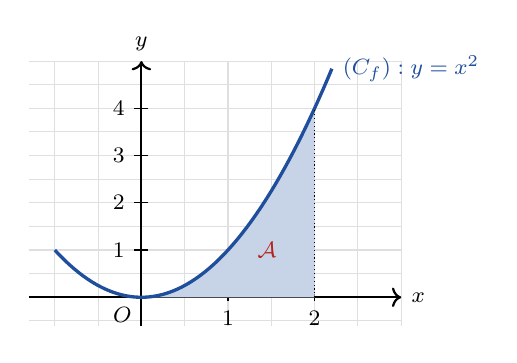
\begin{tikzpicture}[x=1.1cm,y=0.6cm,font=\footnotesize]\draw[gray!25,step=0.5] (-1.3,-0.6) grid (3,5);\draw[->,thick] (-1.3,0)--(3,0) node[right]{$x$}; \draw[->,thick] (0,-0.6)--(0,5) node[above]{$y$};\draw (1,0.08)--(1,-0.08) node[below]{$1$};\draw (2,0.08)--(2,-0.08) node[below]{$2$};\draw (0.08,1)--(-0.08,1) node[left]{$1$};\draw (0.08,2)--(-0.08,2) node[left]{$2$};\draw (0.08,3)--(-0.08,3) node[left]{$3$};\draw (0.08,4)--(-0.08,4) node[left]{$4$};\node[below left] at (0,0){$O$};\fill[cDef!25] (0,0) -- plot[domain=0:2,samples=50] (\x,{\x*\x}) -- (2,0) -- cycle;
\draw[cDef,very thick,domain=-1:2.2,samples=60] plot (\x,{\x*\x}) node[right]{$(C_f):y=x^2$};
\draw[densely dotted] (2,0)--(2,4); \node[cThm] at (1.45,1){$\mathcal A$};\end{tikzpicture}\end{LTR}\par $\displaystyle\int_{0}^{2}x^2\,\mathrm dx=\left[\dfrac{x^3}3\right]_0^2=\dfrac83-0=\RR{\dfrac83\ \mathrm{u.a}}$.}{}{}
\Row{}{%
\Lab{cThm!80!black}{حذار}\ وحدة المساحات $\mathrm{u.a}$ تتعلق بوحدتي المعلم.}{}{}
\Row{التقويم}{%
\Lab{cMeth}{تمرين تطبيقي}\par احسب:\par\textbf{(1)} $\displaystyle\int_{1}^{e}\dfrac1x\,\mathrm dx$.\par\textbf{(2)} $\displaystyle\int_{0}^{\frac\pi2}\cos x\,\mathrm dx$.\par\textbf{(3)} $\displaystyle\int_{0}^{1}e^{2x}\,\mathrm dx$.}{25 د}{تقويم فردي.}
\Row{}{%
\Lab{cEx}{حل التمرين التطبيقي}\par\textbf{(1)} $\big[\ln x\big]_1^e=1-0=\RR{1}$.\par\textbf{(2)} $\big[\sin x\big]_0^{\frac\pi2}=1-0=\RR{1}$.\par\textbf{(3)} $\left[\dfrac12e^{2x}\right]_0^1=\RR{\dfrac{e^2-1}2}$.\par\textbf{واجب منزلي:} تمرين 10 صفحة 184 ، وتمارين 11 إلى 14 صفحتي 183 و 184.\par\smallskip\textbf{ملاحظات حول سير الحصة:} \dotfill}{}{}
\end{Sayr}
\newpage
\ModhHead{41}{3 ع ت}{تحليل}{الدوال الأصلية والحساب التكاملي}{02 سا}{خواص التكامل ، مساحة حيز بين منحنيين}%
{\begin{itemize}\item تعريف التكامل.\end{itemize}}%
{\begin{itemize}\item استعمال خواص التكامل.\item حساب مساحة حيز بين منحنيين.\end{itemize}}%
{المنهاج ، الكتاب المدرسي (الجزء الأول) ، الآلة الحاسبة البيانية ، برمجية Geogebra.}
\begin{Sayr}
\Row{مرحلة الانطلاق}{%
\textbf{التهيئة النفسية:} كيف نحسب المساحة بين منحنيي $y=x$ و $y=x^2$ ؟}{10 د}{سؤال.}
\Row{التشخيص والاكتشاف}{%
\Lab{cEx}{نشاط رقم 06}\ $f(x)=x$ و $g(x)=x^2$ على $[0;1]$.\par\textbf{(1)} ادرس إشارة $f(x)-g(x)$ على $[0;1]$.\par\textbf{(2)} احسب $\displaystyle\int_{0}^{1}x\,\mathrm dx$ و $\displaystyle\int_{0}^{1}x^2\,\mathrm dx$ ، ثم الفرق.}{35 د}{جدول الوضع النسبي ثم الرسم.}
\Row{}{%
\Lab{cDef}{مناقشة النشاط}\par\textbf{(1)} $f(x)-g(x)=x(1-x)\geqslant0$ على $[0;1]$: $(C_f)$ \RR{فوق} $(C_g)$.\par\textbf{(2)} $\dfrac12-\dfrac13=\RR{\dfrac16}$: هو مساحة الحيز بين المنحنيين.}{}{}
\Row{بناء المعارف}{%
\Lab{cThm}{خواص التكامل}\par\textbf{(1)} \textbf{الخطية}: $\RR{\int_a^b(\alpha f+\beta g)=\alpha\int_a^bf+\beta\int_a^bg}$.\par\textbf{(2)} \textbf{علاقة شال}: $\RR{\int_a^cf=\int_a^bf+\int_b^cf}$ ؛ $\int_a^af=0$ ؛ $\int_b^af=-\int_a^bf$.\par\textbf{(3)} \textbf{الترتيب} ($a\leqslant b$): إذا كان $f\geqslant0$ فإن $\int_a^bf\geqslant0$ ؛ إذا كان $f\leqslant g$ فإن $\int_a^bf\leqslant\int_a^bg$.}{50 د}{تلوين الحيز.}
\Row{}{%
\Lab{cThm}{مساحة حيز بين منحنيين}\ إذا كان $(C_f)$ فوق $(C_g)$ على $[a;b]$: $\RR{\mathcal A=\displaystyle\int_{a}^{b}\big(f(x)-g(x)\big)\,\mathrm dx}$.}{}{}
\Row{}{%
\Lab{cEx}{مثال: الوضع النسبي أولًا ثم الرسم}\par\smallskip\begin{LTR}\centering \begin{tikzpicture}[font=\normalsize]
\fill[gray!12] (0,0) rectangle (2.6,-0.9);
\fill[green!18] (2.6,0) rectangle (12.5,-0.9);
\fill[orange!45] (0,-0.9) rectangle (2.6,-4.6);
\fill[cyan!22] (2.6,-0.9) rectangle (12.5,-4.6);
\draw[thick] (0,0) rectangle (12.5,-4.6); \draw (0,-0.9)--(12.5,-0.9) (0,-1.8)--(12.5,-1.8) (2.6,0)--(2.6,-4.6);
\node at (1.3,-0.45){$x$};
\node at (1.3,-1.35){$x-x^2$};
\node[align=center,font=\bfseries] at (1.3,-3.2){\ar{الوضع}\\ \ar{النسبي}};
\node at (4.8,-0.45){$0$};
\node at (10.3,-0.45){$1$};
\node at (7.55,-1.35){$+$};
\node[align=center,font=\small] at (7.55,-3.2){$(C_f)$\\ \ar{فوق}\\ $(C_g)$};
\node at (4.8,-1.35){$0$};
\draw[densely dotted] (4.8,-0.9)--(4.8,-1.13) (4.8,-1.57)--(4.8,-1.8);
\draw (3.3,-4.6) .. controls (3.375,-3.06) and (4.35,-2.136) .. (4.8,-1.8) .. controls (5.25,-2.136) and (6.225,-3.06) .. (6.3,-4.6);
\node[align=center,font=\footnotesize,inner sep=0pt] at (4.8,-3.65){\ar{$(C_f)$ يقطع}\\ $(C_g)$\\ \ar{في النقطة}\\ $O(0;0)$};
\node at (10.3,-1.35){$0$};
\draw[densely dotted] (10.3,-0.9)--(10.3,-1.13) (10.3,-1.57)--(10.3,-1.8);
\draw (8.8,-4.6) .. controls (8.875,-3.06) and (9.85,-2.136) .. (10.3,-1.8) .. controls (10.75,-2.136) and (11.725,-3.06) .. (11.8,-4.6);
\node[align=center,font=\footnotesize,inner sep=0pt] at (10.3,-3.65){\ar{$(C_f)$ يقطع}\\ $(C_g)$\\ \ar{في النقطة}\\ $A(1;1)$};
\end{tikzpicture}\end{LTR}\par \par\smallskip\begin{LTR}\centering 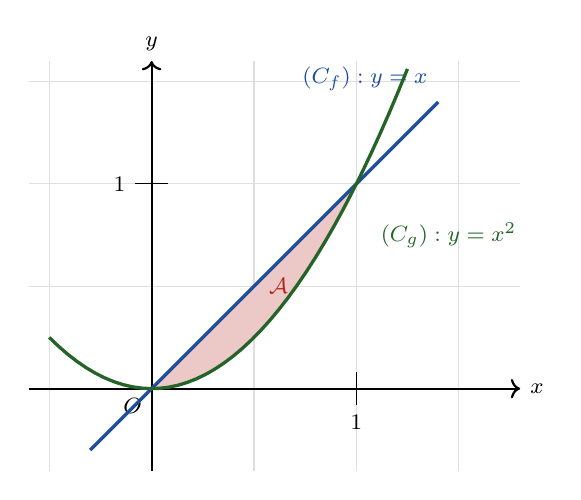
\begin{tikzpicture}[x=2.6cm,y=2.6cm,font=\footnotesize]\draw[gray!25,step=0.5] (-0.6,-0.4) grid (1.8,1.6);\draw[->,thick] (-0.6,0)--(1.8,0) node[right]{$x$}; \draw[->,thick] (0,-0.4)--(0,1.6) node[above]{$y$};\draw (1,0.08)--(1,-0.08) node[below]{$1$};\draw (0.08,1)--(-0.08,1) node[left]{$1$};\node[below left] at (0,0){$O$};\fill[cThm!25] plot[domain=0:1,samples=40] (\x,\x) -- plot[domain=1:0,samples=40] (\x,{\x*\x}) -- cycle;
\draw[cDef,very thick] (-0.3,-0.3)--(1.4,1.4) node[above left]{$(C_f):y=x$};
\draw[cRem!80!black,very thick,domain=-0.5:1.25,samples=40] plot (\x,{\x*\x}); \node[cRem!80!black] at (1.45,0.75){$(C_g):y=x^2$};
\node[cThm] at (0.62,0.5){$\mathcal A$};\end{tikzpicture}\end{LTR}\par $\mathcal A=\displaystyle\int_{0}^{1}(x-x^2)\,\mathrm dx=\left[\dfrac{x^2}2-\dfrac{x^3}3\right]_0^1=\RR{\dfrac16\ \mathrm{u.a}}$.}{}{}
\Row{}{%
\Lab{cThm!80!black}{حذار}\ ندرس إشارة الفرق قبل الحساب ، ونطرح الأسفل من الأعلى.}{}{}
\Row{التقويم}{%
\Lab{cMeth}{تمرين تطبيقي}\par\par\textbf{(1)} احسب بالخطية $I=\displaystyle\int_{0}^{1}(2x+3e^x)\,\mathrm dx$.\par\textbf{(2)} احسب مساحة الحيز المحصور بين $y=x^2$ و $y=2x$.}{25 د}{تقويم فردي.}
\Row{}{%
\Lab{cEx}{حل التمرين التطبيقي}\par\textbf{(1)} $I=2\times\dfrac12+3(e-1)=\RR{3e-2}$.\par\textbf{(2)} التقاطع: $x^2=2x\iff x=0$ أو $x=2$ ؛ $2x-x^2=x(2-x)\geqslant0$ على $[0;2]$:\par\smallskip\begin{LTR}\centering \begin{tikzpicture}[font=\normalsize]
\fill[gray!12] (0,0) rectangle (2.6,-0.9);
\fill[green!18] (2.6,0) rectangle (12.5,-0.9);
\fill[orange!45] (0,-0.9) rectangle (2.6,-4.6);
\fill[cyan!22] (2.6,-0.9) rectangle (12.5,-4.6);
\draw[thick] (0,0) rectangle (12.5,-4.6); \draw (0,-0.9)--(12.5,-0.9) (0,-1.8)--(12.5,-1.8) (2.6,0)--(2.6,-4.6);
\node at (1.3,-0.45){$x$};
\node at (1.3,-1.35){$2x-x^2$};
\node[align=center,font=\bfseries] at (1.3,-3.2){\ar{الوضع}\\ \ar{النسبي}};
\node at (4.8,-0.45){$0$};
\node at (10.3,-0.45){$2$};
\node at (7.55,-1.35){$+$};
\node[align=center,font=\small] at (7.55,-3.2){$(y=2x)$\\ \ar{فوق}\\ $(y=x^2)$};
\node at (4.8,-1.35){$0$};
\draw[densely dotted] (4.8,-0.9)--(4.8,-1.13) (4.8,-1.57)--(4.8,-1.8);
\draw (3.3,-4.6) .. controls (3.375,-3.06) and (4.35,-2.136) .. (4.8,-1.8) .. controls (5.25,-2.136) and (6.225,-3.06) .. (6.3,-4.6);
\node[align=center,font=\footnotesize,inner sep=0pt] at (4.8,-3.65){\ar{$(y=2x)$ يقطع}\\ $(y=x^2)$\\ \ar{في النقطة}\\ $O(0;0)$};
\node at (10.3,-1.35){$0$};
\draw[densely dotted] (10.3,-0.9)--(10.3,-1.13) (10.3,-1.57)--(10.3,-1.8);
\draw (8.8,-4.6) .. controls (8.875,-3.06) and (9.85,-2.136) .. (10.3,-1.8) .. controls (10.75,-2.136) and (11.725,-3.06) .. (11.8,-4.6);
\node[align=center,font=\footnotesize,inner sep=0pt] at (10.3,-3.65){\ar{$(y=2x)$ يقطع}\\ $(y=x^2)$\\ \ar{في النقطة}\\ $A(2;4)$};
\end{tikzpicture}\end{LTR}\par \par\smallskip\begin{LTR}\centering 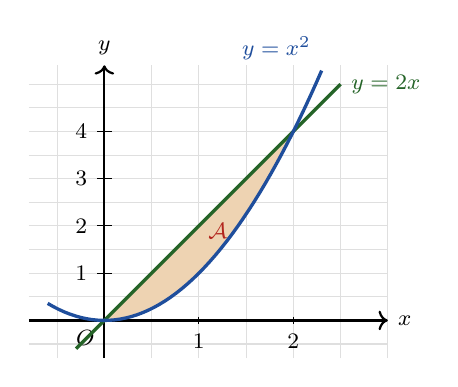
\begin{tikzpicture}[x=1.2cm,y=0.6cm,font=\footnotesize]\draw[gray!25,step=0.5] (-0.8,-0.8) grid (3,5.4);\draw[->,thick] (-0.8,0)--(3,0) node[right]{$x$}; \draw[->,thick] (0,-0.8)--(0,5.4) node[above]{$y$};\draw (1,0.08)--(1,-0.08) node[below]{$1$};\draw (2,0.08)--(2,-0.08) node[below]{$2$};\draw (0.08,1)--(-0.08,1) node[left]{$1$};\draw (0.08,2)--(-0.08,2) node[left]{$2$};\draw (0.08,3)--(-0.08,3) node[left]{$3$};\draw (0.08,4)--(-0.08,4) node[left]{$4$};\node[below left] at (0,0){$O$};\fill[cEx!30] plot[domain=0:2,samples=10] (\x,{2*\x}) -- plot[domain=2:0,samples=40] (\x,{\x*\x}) -- cycle;
\draw[cRem!80!black,very thick] (-0.3,-0.6)--(2.5,5) node[right]{$y=2x$};
\draw[cDef,very thick,domain=-0.6:2.3,samples=50] plot (\x,{\x*\x}) node[above left]{$y=x^2$};
\node[cThm] at (1.2,1.9){$\mathcal A$};\end{tikzpicture}\end{LTR}\par $\mathcal A=\displaystyle\int_{0}^{2}(2x-x^2)\,\mathrm dx=\left[x^2-\dfrac{x^3}3\right]_0^2=4-\dfrac83=\RR{\dfrac43\ \mathrm{u.a}}$.\par\textbf{واجب منزلي:} تمارين 30 إلى 33 صفحة 186.\par\smallskip\textbf{ملاحظات حول سير الحصة:} \dotfill}{}{}
\end{Sayr}
\newpage
\ModhHead{42}{3 ع ت}{تحليل}{الدوال الأصلية والحساب التكاملي}{02 سا}{القيمة المتوسطة لدالة على مجال ، حصر تكامل}%
{\begin{itemize}\item خواص التكامل.\end{itemize}}%
{\begin{itemize}\item حساب القيمة المتوسطة لدالة وتفسيرها.\item حصر تكامل.\end{itemize}}%
{المنهاج ، الكتاب المدرسي (الجزء الأول) ، الآلة الحاسبة البيانية ، برمجية Geogebra.}
\begin{Sayr}
\Row{مرحلة الانطلاق}{%
\textbf{التهيئة النفسية:} درجات الحرارة خلال يوم تتغير باستمرار: ما معنى «الحرارة المتوسطة»؟}{10 د}{وضعية مناخية.}
\Row{التشخيص والاكتشاف}{%
\Lab{cEx}{نشاط رقم 07}\ $f(x)=x^2$ على $[0;3]$.\par\textbf{(1)} احسب $\displaystyle\int_{0}^{3}x^2\,\mathrm dx$.\par\textbf{(2)} عيّن ارتفاع مستطيل قاعدته $[0;3]$ وله نفس المساحة.}{35 د}{تفسير هندسي.}
\Row{}{%
\Lab{cDef}{مناقشة النشاط}\par\textbf{(1)} $\left[\dfrac{x^3}3\right]_0^3=\RR{9}$.\par\textbf{(2)} $3\times h=9$ ، إذن $h=\RR{3}$: هي \textbf{القيمة المتوسطة} لـ $f$ على $[0;3]$.}{}{}
\Row{بناء المعارف}{%
\Lab{cDef}{تعريف}\ القيمة المتوسطة لـ $f$ على $[a;b]$ ($a<b$): $\RR{\mu=\dfrac1{b-a}\displaystyle\int_{a}^{b}f(x)\,\mathrm dx}$.}{50 د}{الحصر.}
\Row{}{%
\Lab{cThm}{الحصر}\ إذا كان $m\leqslant f(x)\leqslant M$ على $[a;b]$ فإن: $\RR{m(b-a)\leqslant\displaystyle\int_{a}^{b}f(x)\,\mathrm dx\leqslant M(b-a)}$.}{}{}
\Row{}{%
\Lab{cEx}{أمثلة محلولة}\par\textbf{(1)} القيمة المتوسطة لـ $e^x$ على $[0;1]$: $\mu=\dfrac11\big[e^x\big]_0^1=\RR{e-1}$.\par\textbf{(2)} من أجل $x\in[0;1]$: $0\leqslant x^2\leqslant1$ ، إذن $1\leqslant e^{x^2}\leqslant e$ ، ومنه $\RR{1\leqslant\displaystyle\int_{0}^{1}e^{x^2}\,\mathrm dx\leqslant e}$.}{}{}
\Row{}{%
\Lab{cThm!80!black}{حذار}\ لا نستطيع حساب $\int e^{x^2}$ بدالة أصلية مألوفة: الحصر هو الحل.}{}{}
\Row{التقويم}{%
\Lab{cMeth}{تمرين تطبيقي}\par\par\textbf{(1)} احسب القيمة المتوسطة لـ $\sin$ على $[0;\pi]$.\par\textbf{(2)} بيّن أن $\dfrac12\leqslant\displaystyle\int_{0}^{1}\dfrac1{1+x^2}\,\mathrm dx\leqslant1$.}{25 د}{تقويم فردي.}
\Row{}{%
\Lab{cEx}{حل التمرين التطبيقي}\par\textbf{(1)} $\mu=\dfrac1\pi\big[-\cos x\big]_0^\pi=\dfrac1\pi(1+1)=\RR{\dfrac2\pi}$.\par\textbf{(2)} على $[0;1]$: $1\leqslant1+x^2\leqslant2$ ، إذن $\dfrac12\leqslant\dfrac1{1+x^2}\leqslant1$ ، وبالحصر (الطول $1$) نحصل على \RR{المطلوب}.\par\textbf{واجب منزلي:} تمرين 36 صفحة 186 ، وتمرين 51 صفحة 188.\par\smallskip\textbf{ملاحظات حول سير الحصة:} \dotfill}{}{}
\end{Sayr}
\newpage
\ModhHead{43}{3 ع ت}{تحليل}{الدوال الأصلية والحساب التكاملي}{02 سا}{حساب مساحة حيز: حالة دالة سالبة أو متغيرة الإشارة}%
{\begin{itemize}\item التكامل ، الوضع النسبي.\end{itemize}}%
{\begin{itemize}\item حساب مساحة حيز يقع تحت محور الفواصل أو على جانبيه.\end{itemize}}%
{المنهاج ، الكتاب المدرسي (الجزء الأول) ، الآلة الحاسبة البيانية ، برمجية Geogebra.}
\begin{Sayr}
\Row{مرحلة الانطلاق}{%
\textbf{التهيئة النفسية:} ما إشارة $\displaystyle\int_{-2}^{2}(x^2-4)\,\mathrm dx$ ؟ هل المساحة سالبة؟}{10 د}{سؤال إشكالي.}
\Row{التشخيص والاكتشاف}{%
\Lab{cEx}{نشاط رقم 08}\ $f(x)=x^2-4$ على $[-2;2]$.\par\textbf{(1)} ادرس إشارة $f(x)$ على $[-2;2]$.\par\textbf{(2)} احسب $\displaystyle\int_{-2}^{2}f(x)\,\mathrm dx$ ، وقارنه بالمساحة.}{35 د}{جدول الوضع النسبي.}
\Row{}{%
\Lab{cDef}{مناقشة النشاط}\par\textbf{(1)} $f(x)=(x-2)(x+2)\leqslant0$ على $[-2;2]$: $(C_f)$ \RR{تحت} محور الفواصل.\par\textbf{(2)} $\left[\dfrac{x^3}3-4x\right]_{-2}^2=\left(\dfrac83-8\right)-\left(-\dfrac83+8\right)=\RR{-\dfrac{32}3}$: التكامل سالب ، والمساحة \RR{$\dfrac{32}3$}.}{}{}
\Row{بناء المعارف}{%
\Lab{cThm}{خاصية}\par\textbf{(1)} إذا كانت $f\leqslant0$ على $[a;b]$: $\RR{\mathcal A=-\displaystyle\int_{a}^{b}f(x)\,\mathrm dx}$.\par\textbf{(2)} إذا تغيرت الإشارة: نقسم المجال عند الأصفار (علاقة شال) ونجمع المساحات.}{50 د}{تلوين الحيز بلونين.}
\Row{}{%
\Lab{cEx}{مثال 1: الوضع النسبي ثم الرسم}\par\smallskip\begin{LTR}\centering \begin{tikzpicture}[font=\normalsize]
\fill[gray!12] (0,0) rectangle (2.6,-0.9);
\fill[green!18] (2.6,0) rectangle (12.5,-0.9);
\fill[orange!45] (0,-0.9) rectangle (2.6,-4.6);
\fill[cyan!22] (2.6,-0.9) rectangle (12.5,-4.6);
\draw[thick] (0,0) rectangle (12.5,-4.6); \draw (0,-0.9)--(12.5,-0.9) (0,-1.8)--(12.5,-1.8) (2.6,0)--(2.6,-4.6);
\node at (1.3,-0.45){$x$};
\node at (1.3,-1.35){$x^2-4$};
\node[align=center,font=\bfseries] at (1.3,-3.2){\ar{الوضع}\\ \ar{النسبي}};
\node at (4.8,-0.45){$-2$};
\node at (10.3,-0.45){$2$};
\node at (7.55,-1.35){$-$};
\node[align=center,font=\small] at (7.55,-3.2){$(C_f)$\\ \ar{تحت}\\ $(xx')$};
\node at (4.8,-1.35){$0$};
\draw[densely dotted] (4.8,-0.9)--(4.8,-1.13) (4.8,-1.57)--(4.8,-1.8);
\draw (3.3,-4.6) .. controls (3.375,-3.06) and (4.35,-2.136) .. (4.8,-1.8) .. controls (5.25,-2.136) and (6.225,-3.06) .. (6.3,-4.6);
\node[align=center,font=\footnotesize,inner sep=0pt] at (4.8,-3.65){\ar{$(C_f)$ يقطع}\\ $(xx')$\\ \ar{في النقطة}\\ $A(-2;0)$};
\node at (10.3,-1.35){$0$};
\draw[densely dotted] (10.3,-0.9)--(10.3,-1.13) (10.3,-1.57)--(10.3,-1.8);
\draw (8.8,-4.6) .. controls (8.875,-3.06) and (9.85,-2.136) .. (10.3,-1.8) .. controls (10.75,-2.136) and (11.725,-3.06) .. (11.8,-4.6);
\node[align=center,font=\footnotesize,inner sep=0pt] at (10.3,-3.65){\ar{$(C_f)$ يقطع}\\ $(xx')$\\ \ar{في النقطة}\\ $B(2;0)$};
\end{tikzpicture}\end{LTR}\par \par\smallskip\begin{LTR}\centering 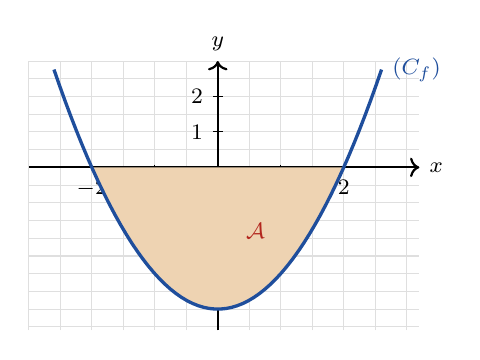
\begin{tikzpicture}[x=0.8cm,y=0.45cm,font=\footnotesize]\draw[gray!25,step=0.5] (-3,-4.6) grid (3.2,3);\draw[->,thick] (-3,0)--(3.2,0) node[right]{$x$}; \draw[->,thick] (0,-4.6)--(0,3) node[above]{$y$};\draw (-2,0.08)--(-2,-0.08) node[below]{$-2$};\draw (-1,0.08)--(-1,-0.08) node[below]{$-1$};\draw (1,0.08)--(1,-0.08) node[below]{$1$};\draw (2,0.08)--(2,-0.08) node[below]{$2$};\draw (0.08,-3)--(-0.08,-3) node[left]{$-3$};\draw (0.08,-2)--(-0.08,-2) node[left]{$-2$};\draw (0.08,-1)--(-0.08,-1) node[left]{$-1$};\draw (0.08,1)--(-0.08,1) node[left]{$1$};\draw (0.08,2)--(-0.08,2) node[left]{$2$};\node[below left] at (0,0){$O$};\fill[cEx!30] (-2,0) -- plot[domain=-2:2,samples=50] (\x,{\x*\x-4}) -- (2,0) -- cycle;
\draw[cDef,very thick,domain=-2.6:2.6,samples=60] plot (\x,{\x*\x-4}) node[right]{$(C_f)$};
\node[cThm] at (0.6,-1.8){$\mathcal A$};\end{tikzpicture}\end{LTR}\par $\mathcal A=-\displaystyle\int_{-2}^{2}(x^2-4)\,\mathrm dx=\RR{\dfrac{32}3\ \mathrm{u.a}}$.}{}{}
\Row{}{%
\Lab{cEx}{مثال 2: دالة متغيرة الإشارة}\ $f(x)=x^2-1$ على $[0;2]$:\par\smallskip\begin{LTR}\centering \begin{tikzpicture}[font=\normalsize]
\fill[gray!12] (0,0) rectangle (2.6,-0.9);
\fill[green!18] (2.6,0) rectangle (12.5,-0.9);
\fill[orange!45] (0,-0.9) rectangle (2.6,-4.6);
\fill[cyan!22] (2.6,-0.9) rectangle (12.5,-4.6);
\draw[thick] (0,0) rectangle (12.5,-4.6); \draw (0,-0.9)--(12.5,-0.9) (0,-1.8)--(12.5,-1.8) (2.6,0)--(2.6,-4.6);
\node at (1.3,-0.45){$x$};
\node at (1.3,-1.35){$x^2-1$};
\node[align=center,font=\bfseries] at (1.3,-3.2){\ar{الوضع}\\ \ar{النسبي}};
\node at (3.3,-0.45){$0$};
\node at (7.55,-0.45){$1$};
\node at (11.8,-0.45){$2$};
\node at (4.675,-1.35){$-$};
\node[align=center,font=\small] at (4.675,-3.2){$(C_f)$\\ \ar{تحت}\\ $(xx')$};
\node at (10.425,-1.35){$+$};
\node[align=center,font=\small] at (10.425,-3.2){$(C_f)$\\ \ar{فوق}\\ $(xx')$};
\node at (7.55,-1.35){$0$};
\draw[densely dotted] (7.55,-0.9)--(7.55,-1.13) (7.55,-1.57)--(7.55,-1.8);
\draw (6.05,-4.6) .. controls (6.125,-3.06) and (7.1,-2.136) .. (7.55,-1.8) .. controls (8,-2.136) and (8.975,-3.06) .. (9.05,-4.6);
\node[align=center,font=\footnotesize,inner sep=0pt] at (7.55,-3.65){\ar{$(C_f)$ يقطع}\\ $(xx')$\\ \ar{في النقطة}\\ $A(1;0)$};
\end{tikzpicture}\end{LTR}\par \par\smallskip\begin{LTR}\centering 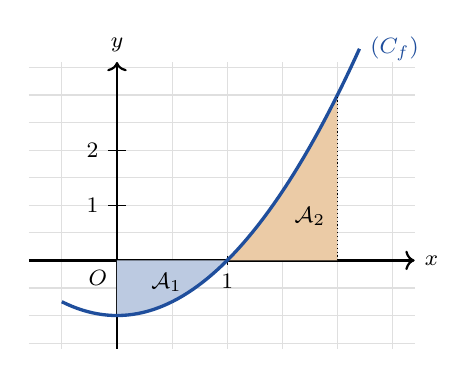
\begin{tikzpicture}[x=1.4cm,y=0.7cm,font=\footnotesize]\draw[gray!25,step=0.5] (-0.8,-1.6) grid (2.7,3.6);\draw[->,thick] (-0.8,0)--(2.7,0) node[right]{$x$}; \draw[->,thick] (0,-1.6)--(0,3.6) node[above]{$y$};\draw (1,0.08)--(1,-0.08) node[below]{$1$};\draw (0.08,1)--(-0.08,1) node[left]{$1$};\draw (0.08,2)--(-0.08,2) node[left]{$2$};\node[below left] at (0,0){$O$};\fill[cDef!30] (0,0) -- plot[domain=0:1,samples=40] (\x,{\x*\x-1}) -- cycle;
\fill[cEx!35] (1,0) -- plot[domain=1:2,samples=40] (\x,{\x*\x-1}) -- (2,0) -- cycle;
\draw[cDef,very thick,domain=-0.5:2.2,samples=60] plot (\x,{\x*\x-1}) node[right]{$(C_f)$};
\draw[densely dotted] (2,0)--(2,3); \node at (0.45,-0.4){$\mathcal A_1$}; \node at (1.75,0.8){$\mathcal A_2$};\end{tikzpicture}\end{LTR}\par \par\textbf{(1)} $\mathcal A_1=-\displaystyle\int_{0}^{1}(x^2-1)\,\mathrm dx=-\left(\dfrac13-1\right)=\RR{\dfrac23}$.\par\textbf{(2)} $\mathcal A_2=\displaystyle\int_{1}^{2}(x^2-1)\,\mathrm dx=\left(\dfrac83-2\right)-\left(\dfrac13-1\right)=\RR{\dfrac43}$ ؛ $\mathcal A=\RR{2\ \mathrm{u.a}}$.}{}{}
\Row{}{%
\Lab{cThm!80!black}{حذار}\ المساحة دائمًا موجبة.}{}{}
\Row{التقويم}{%
\Lab{cMeth}{تمرين تطبيقي}\par احسب مساحة الحيز بين منحنى $\sin$ ومحور الفواصل على $[0;2\pi]$.}{25 د}{تقويم فردي.}
\Row{}{%
\Lab{cEx}{حل التمرين التطبيقي}\par\smallskip\begin{LTR}\centering \begin{tikzpicture}[font=\normalsize]
\fill[gray!12] (0,0) rectangle (2.6,-0.9);
\fill[green!18] (2.6,0) rectangle (12.5,-0.9);
\fill[orange!45] (0,-0.9) rectangle (2.6,-4.6);
\fill[cyan!22] (2.6,-0.9) rectangle (12.5,-4.6);
\draw[thick] (0,0) rectangle (12.5,-4.6); \draw (0,-0.9)--(12.5,-0.9) (0,-1.8)--(12.5,-1.8) (2.6,0)--(2.6,-4.6);
\node at (1.3,-0.45){$x$};
\node at (1.3,-1.35){$\sin x$};
\node[align=center,font=\bfseries] at (1.3,-3.2){\ar{الوضع}\\ \ar{النسبي}};
\node at (4.35,-0.45){$0$};
\node at (7.55,-0.45){$\pi$};
\node at (10.75,-0.45){$2\pi$};
\node at (5.95,-1.35){$+$};
\node[align=center,font=\footnotesize] at (5.95,-3.2){$(C)$\\ \ar{فوق}\\ $(xx')$};
\node at (9.15,-1.35){$-$};
\node[align=center,font=\footnotesize] at (9.15,-3.2){$(C)$\\ \ar{تحت}\\ $(xx')$};
\node at (4.35,-1.35){$0$};
\draw[densely dotted] (4.35,-0.9)--(4.35,-1.13) (4.35,-1.57)--(4.35,-1.8);
\draw (3.3,-4.6) .. controls (3.3525,-3.06) and (4.035,-2.136) .. (4.35,-1.8) .. controls (4.665,-2.136) and (5.3475,-3.06) .. (5.4,-4.6);
\node[align=center,font=\scriptsize,inner sep=0pt] at (4.35,-3.65){\ar{$(C)$ يقطع}\\ $(xx')$\\ \ar{في النقطة}\\ $O(0;0)$};
\node at (7.55,-1.35){$0$};
\draw[densely dotted] (7.55,-0.9)--(7.55,-1.13) (7.55,-1.57)--(7.55,-1.8);
\draw (6.5,-4.6) .. controls (6.5525,-3.06) and (7.235,-2.136) .. (7.55,-1.8) .. controls (7.865,-2.136) and (8.5475,-3.06) .. (8.6,-4.6);
\node[align=center,font=\scriptsize,inner sep=0pt] at (7.55,-3.65){\ar{$(C)$ يقطع}\\ $(xx')$\\ \ar{في النقطة}\\ $A(\pi;0)$};
\node at (10.75,-1.35){$0$};
\draw[densely dotted] (10.75,-0.9)--(10.75,-1.13) (10.75,-1.57)--(10.75,-1.8);
\draw (9.7,-4.6) .. controls (9.7525,-3.06) and (10.435,-2.136) .. (10.75,-1.8) .. controls (11.065,-2.136) and (11.7475,-3.06) .. (11.8,-4.6);
\node[align=center,font=\scriptsize,inner sep=0pt] at (10.75,-3.65){\ar{$(C)$ يقطع}\\ $(xx')$\\ \ar{في النقطة}\\ $B(2\pi;0)$};
\end{tikzpicture}\end{LTR}\par \par\textbf{(1)} $\mathcal A_1=\displaystyle\int_{0}^{\pi}\sin x\,\mathrm dx=\big[-\cos x\big]_0^\pi=\RR{2}$.\par\textbf{(2)} $\mathcal A_2=-\displaystyle\int_{\pi}^{2\pi}\sin x\,\mathrm dx=-\big[-\cos x\big]_\pi^{2\pi}=\RR{2}$ ؛ $\mathcal A=\RR{4\ \mathrm{u.a}}$.\par\textbf{واجب منزلي:} تمارين 52 إلى 59 صفحتي 188 و 189.\par\smallskip\textbf{ملاحظات حول سير الحصة:} \dotfill}{}{}
\end{Sayr}
\newpage
\ModhHead{44}{3 ع ت}{تحليل}{الدوال الأصلية والحساب التكاملي}{02 سا}{التكامل بالتجزئة ، توظيف التكامل لحساب دوال أصلية}%
{\begin{itemize}\item خواص التكامل ، مشتقة جداء.\end{itemize}}%
{\begin{itemize}\item حساب تكاملات بالتجزئة.\item تعيين دوال أصلية بالتكامل.\end{itemize}}%
{المنهاج ، الكتاب المدرسي (الجزء الأول) ، الآلة الحاسبة البيانية ، برمجية Geogebra.}
\begin{Sayr}
\Row{مرحلة الانطلاق}{%
\textbf{التهيئة النفسية:} كيف نحسب $\displaystyle\int_{0}^{1}xe^x\,\mathrm dx$ ؟ لا يوجد في الجدول.}{10 د}{سؤال.}
\Row{التشخيص والاكتشاف}{%
\Lab{cEx}{نشاط رقم 09}\par\textbf{(1)} اكتب مشتقة الجداء $uv$.\par\textbf{(2)} كامل طرفي المساواة على $[a;b]$ واستنتج دستورًا.}{35 د}{مشتقة الجداء.}
\Row{}{%
\Lab{cDef}{مناقشة النشاط}\par\textbf{(1)} $(uv)^{\prime}=u^{\prime}v+uv^{\prime}$.\par\textbf{(2)} $\big[uv\big]_a^b=\int_a^bu^{\prime}v+\int_a^buv^{\prime}$ ، ومنه $\RR{\int_a^buv^{\prime}=\big[uv\big]_a^b-\int_a^bu^{\prime}v}$.}{}{}
\Row{بناء المعارف}{%
\Lab{cThm}{التكامل بالتجزئة}\ $u$ و $v$ قابلتان للاشتقاق ومشتقتاهما مستمرتان: $\RR{\displaystyle\int_{a}^{b}u(x)v^{\prime}(x)\,\mathrm dx=\big[u(x)v(x)\big]_a^b-\displaystyle\int_{a}^{b}u^{\prime}(x)v(x)\,\mathrm dx}$.}{50 د}{اختيار $u$ و $v^{\prime}$.}
\Row{}{%
\Lab{cEx}{أمثلة محلولة}\par\textbf{(1)} $\displaystyle\int_{0}^{1}xe^x\,\mathrm dx$: $u=x$ ، $v^{\prime}=e^x$ ، $u^{\prime}=1$ ، $v=e^x$:\par $=\big[xe^x\big]_0^1-\displaystyle\int_{0}^{1}e^x\,\mathrm dx=e-(e-1)=\RR{1}$.\par\textbf{(2)} $\displaystyle\int_{1}^{e}\ln x\,\mathrm dx$: $u=\ln x$ ، $v^{\prime}=1$ ، $v=x$:\par $=\big[x\ln x\big]_1^e-\displaystyle\int_{1}^{e}1\,\mathrm dx=e-(e-1)=\RR{1}$.}{}{}
\Row{}{%
\Lab{cThm}{دالة أصلية بالتكامل}\ $x\mapsto\displaystyle\int_a^xf(t)\,\mathrm dt$ هي \RR{الدالة} \RR{الأصلية} \RR{لـ} \RR{$f$} \RR{التي} \RR{تنعدم} \RR{عند} \RR{$a$}. مثال: $\displaystyle\int_1^x\ln t\,\mathrm dt=\RR{x\ln x-x+1}$.}{}{}
\Row{}{%
\Lab{cThm!80!black}{حذار}\ نختار $u$ التي تبسط بالاشتقاق ($x$ ، $\ln x$).}{}{}
\Row{التقويم}{%
\Lab{cMeth}{تمرين تطبيقي}\par احسب:\par\textbf{(1)} $\displaystyle\int_{0}^{\pi}x\cos x\,\mathrm dx$.\par\textbf{(2)} $\displaystyle\int_{1}^{e}x\ln x\,\mathrm dx$.}{25 د}{تقويم فردي.}
\Row{}{%
\Lab{cEx}{حل التمرين التطبيقي}\par\textbf{(1)} $u=x$ ، $v^{\prime}=\cos x$ ، $v=\sin x$: $\big[x\sin x\big]_0^\pi-\displaystyle\int_{0}^{\pi}\sin x\,\mathrm dx=0-2=\RR{-2}$.\par\textbf{(2)} $u=\ln x$ ، $v^{\prime}=x$ ، $v=\dfrac{x^2}2$: $\left[\dfrac{x^2}2\ln x\right]_1^e-\displaystyle\int_{1}^{e}\dfrac x2\,\mathrm dx=\dfrac{e^2}2-\dfrac{e^2-1}4=\RR{\dfrac{e^2+1}4}$.\par\textbf{واجب منزلي:} تمارين 62 إلى 65 ، و 68 إلى 70 صفحة 189.\par\smallskip\textbf{ملاحظات حول سير الحصة:} \dotfill}{}{}
\end{Sayr}
\newpage
\ModhHead{45}{3 ع ت}{تحليل}{الدوال الأصلية والحساب التكاملي}{02 سا}{حساب حجوم مجسمات بسيطة ، حل مشكلات}%
{\begin{itemize}\item الحساب التكاملي.\end{itemize}}%
{\begin{itemize}\item حساب حجم مجسم بالتكامل.\item توظيف التكامل في حل مشكلات بسيطة.\end{itemize}}%
{المنهاج ، الكتاب المدرسي (الجزء الأول) ، الآلة الحاسبة البيانية ، برمجية Geogebra.}
\begin{Sayr}
\Row{مرحلة الانطلاق}{%
\textbf{التهيئة النفسية:} كيف نبرهن أن حجم المخروط ثلث حجم الأسطوانة؟}{10 د}{سؤال تاريخي.}
\Row{التشخيص والاكتشاف}{%
\Lab{cEx}{نشاط رقم 10}\ مخروط دوراني نصف قطر قاعدته $r$ وارتفاعه $h$ ، رأسه في $O$ ومحوره محور الفواصل.\par\textbf{(1)} عبّر عن نصف قطر المقطع عند الفاصلة $x$ ($0\leqslant x\leqslant h$).\par\textbf{(2)} استنتج مساحة المقطع $S(x)$.}{35 د}{نموذج حقيقي.}
\Row{}{%
\Lab{cDef}{مناقشة النشاط}\par\textbf{(1)} بتناسب المثلثين: نصف القطر $\RR{\dfrac{rx}h}$.\par\textbf{(2)} $S(x)=\pi\left(\dfrac{rx}h\right)^2=\RR{\dfrac{\pi r^2x^2}{h^2}}$.}{}{}
\Row{بناء المعارف}{%
\Lab{cThm}{خاصية}\par\textbf{(1)} حجم مجسم مساحة مقطعه $S(x)$ على $[a;b]$: $\RR{V=\displaystyle\int_{a}^{b}S(x)\,\mathrm dx}$.\par\textbf{(2)} مجسم دوراني حول محور الفواصل: $\RR{V=\pi\displaystyle\int_{a}^{b}f(x)^2\,\mathrm dx}$.}{50 د}{رسم المقطع.}
\Row{}{%
\Lab{cEx}{أمثلة محلولة}\par\textbf{(1)} المخروط: $V=\displaystyle\int_{0}^{h}\dfrac{\pi r^2x^2}{h^2}\,\mathrm dx=\dfrac{\pi r^2}{h^2}\times\dfrac{h^3}3=\RR{\dfrac{\pi r^2h}3}$.\par\textbf{(2)} الكرة: دوران $f(x)=\sqrt{r^2-x^2}$ على $[-r;r]$: $V=\pi\displaystyle\int_{-r}^{r}(r^2-x^2)\,\mathrm dx=\RR{\dfrac43\pi r^3}$.}{}{}
\Row{}{%
\Lab{cThm!80!black}{حذار}\ وحدة الحجم $\mathrm{u.v}$.}{}{}
\Row{التقويم}{%
\Lab{cMeth}{تمرين تطبيقي}\par احسب حجم المجسم الناتج عن دوران المنحنى حول محور الفواصل:\par\textbf{(1)} $f(x)=\sqrt x$ على $[0;4]$.\par\textbf{(2)} $g(x)=e^x$ على $[0;1]$.}{25 د}{نهاية المحور: فرض أو مراجعة.}
\Row{}{%
\Lab{cEx}{حل التمرين التطبيقي}\par\textbf{(1)} $V=\pi\displaystyle\int_{0}^{4}x\,\mathrm dx=\pi\left[\dfrac{x^2}2\right]_0^4=\RR{8\pi\ \mathrm{u.v}}$.\par\textbf{(2)} $V=\pi\displaystyle\int_{0}^{1}e^{2x}\,\mathrm dx=\RR{\dfrac{\pi\left(e^2-1\right)}2\ \mathrm{u.v}}$.\par\textbf{واجب منزلي:} تمرينا 72 و 73 صفحة 189.\par\smallskip\textbf{ملاحظات حول سير الحصة:} \dotfill}{}{}
\end{Sayr}
\end{document}
